\RequirePackage{fix-cm}
%\documentclass[10pt,a4paper, twoside, titlepage]{article}
\documentclass[11pt,a4paper, titlepage]{article}
\usepackage[latin1]{inputenc}
\usepackage{amsmath}
\usepackage{amsfonts}
\usepackage{amssymb}

\usepackage{fixltx2e}

%\usepackage[pdftex]{graphicx, color}
\usepackage{graphicx}
\usepackage{color}
\usepackage{adjustbox}
\usepackage{pdfpages}
\usepackage{epsfig}

\DeclareGraphicsRule{.pdftex}{pdf}{.pdftex}{}

\usepackage{subfigure}

\usepackage[]{natbib}

\makeatletter

%sequenz-diagramm
\usepackage{tikz}
\usetikzlibrary{positioning}
\usetikzlibrary{arrows,shadows}

%code snippets
%\usepackage{color}
\usepackage{listings}
\usepackage{courier}
\usepackage{caption}
\usepackage{pgf-umlsd}
 \lstset{
         basicstyle=\footnotesize\ttfamily, % Standardschrift
         %numbers=left,               % Ort der Zeilennummern
         numberstyle=\tiny,          % Stil der Zeilennummern
         %stepnumber=2,               % Abstand zwischen den Zeilennummern
         numbersep=5pt,              % Abstand der Nummern zum Text
         tabsize=2,                  % Groesse von Tabs
         extendedchars=true,         %
         breaklines=true,            % Zeilen werden Umgebrochen
         keywordstyle=\color{red},
            frame=b,         
 %        keywordstyle=[1]\textbf,    % Stil der Keywords
 %        keywordstyle=[2]\textbf,    %
 %        keywordstyle=[3]\textbf,    %
 %        keywordstyle=[4]\textbf,   \sqrt{\sqrt{}} %
         stringstyle=\color{white}\ttfamily, % Farbe der String
         showspaces=false,           % Leerzeichen anzeigen ?
         showtabs=false,             % Tabs anzeigen ?
         xleftmargin=17pt,
         framexleftmargin=17pt,
         framexrightmargin=5pt,
         framexbottommargin=4pt,
         %backgroundcolor=\color{lightgray},
         showstringspaces=false      % Leerzeichen in Strings anzeigen ?        
 }
 \lstloadlanguages{% Check Dokumentation for further languages ...
         %[Visual]Basic
         %Pascal
         %C
         C++
         %XML
         %HTML
         %Java
 }
%\DeclareCaptionFont{blue}{\color{blue}} 

%\captionsetup[lstlisting]{singlelinecheck=false, labelfont={blue}, textfont={blue}}
\DeclareCaptionFont{white}{\color{white}}
\DeclareCaptionFormat{listing}{\colorbox[cmyk]{0.43, 0.35, 0.35,0.01}{\parbox{\textwidth}{\hspace{15pt}#1#2#3}}}
\captionsetup[lstlisting]{format=listing,labelfont=white,textfont=white, singlelinecheck=false, margin=0pt, font={bf,footnotesize}}
% code snippets end ############################################

\DeclareRobustCommand{\greektext}{%
  \fontencoding{LGR}\selectfont\def\encodingdefault{LGR}}
\DeclareRobustCommand{\textgreek}[1]{\leavevmode{\greektext #1}}
\DeclareFontEncoding{LGR}{}{}
\DeclareTextSymbol{\~}{LGR}{126}

\numberwithin{equation}{section}
\numberwithin{figure}{section}
\numberwithin{table}{section}

\usepackage{setspace}
\newcommand{\MSonehalfspacing}{%
  \setstretch{1.44}%  default
  \ifcase \@ptsize \relax % 10pt
    \setstretch {1.448}%
  \or % 11pt
    \setstretch {1.399}%
  \or % 12pt
    \setstretch {1.433}%
  \fi
}
\newcommand{\MSdoublespacing}{%
  \setstretch {1.92}%  default
  \ifcase \@ptsize \relax % 10pt
    \setstretch {1.936}%
  \or % 11pt
    \setstretch {1.866}%
  \or % 12pt
    \setstretch {1.902}%
  \fi
}
\MSonehalfspacing


\makeatother

\begin{document}

\title{Automated Routing in Pedestrian Dynamics \newline
Fachhochschule Aachen, Campus Jülich \newline
Medizintechnik und Technomathematik, \newline
Technomathematik \newline
Forschungszentrum Jülich GmbH, JSC, \newline
Civil Security and Traffic}


\author{Masterthesis from Arne Graf}


\date{2015-10-16}
\pagenumbering{gobble}% Remove page numbers (and reset to 1)

\newpage
\begin{titlepage}

\begin{center}

% Oberer Teil der Titelseite:
\includegraphics[width=0.6\linewidth]{pics/Ju}\\[1cm]    

\textsc{\LARGE Forschungszentrum J{\"u}lich GmbH}\\[1.5cm]

\textsc{\Large Masterthesis}\\[0.5cm]


% Title
\newcommand{\HHRule}{\rule{\linewidth}{0.5mm}}
\HHRule \\[0.4cm]
{ \huge \bfseries Automated Routing in Pedestrian Dynamics}\\[0.4cm]
\HHRule \\[1.5cm]

Fachhochschule Aachen, Campus J{\"u}lich

Fachbereich: Medizintechnik und Technomathematik,

Studiengang: Technomathematik

\vfill

% Author and supervisor
\begin{minipage}{0.3\textwidth}
\begin{flushleft} \large
%\emph{\ \\}
%\textsc{\ \\}
\emph{Autor:}\\
Arne \textsc{Graf}
\end{flushleft}
\end{minipage}
\hfill
\begin{minipage}{0.6\textwidth}
\begin{flushright} \large
\emph{Erstpr{\"u}fer:} \\
Prof. Dr. Johannes \textsc{Grotendorst} \\
\emph{Zweitpr{\"u}fer:} \\
Dr. Mohcine \textsc{Chraibi}
\end{flushright}
\end{minipage}

\vfill

% Unterer Teil der Seite
{\large J{\"u}lich, 2015-10-06}

\end{center}

\end{titlepage}
\newpage
%Eigenständigkeitserklärung
\section*{Eigenst{\"a}ndigkeitserkl{\"a}rung}
Diese Arbeit wurde von mir selbstst{\"a}ndig angefertigt und verfasst.
Es sind keine anderen als die angegebenen Quellen und Hilfsmittel
benutzt worden.

%% Abstand und Linie
\vspace{20mm}
\hrule
\vspace{5mm}
\begin{minipage}{0.4\textwidth}
Ort und Datum
\end{minipage}
\hfill
\begin{minipage}{0.6\textwidth}
\begin{flushright}
Unterschrift $\qquad$
\end{flushright}
\end{minipage}
\vspace{7cm}

\begin{flushleft}
\begin{tabular}{lll}
Diese Arbeit & wurde betreut von:  & \\
Erstpr{\"u}fer: & Professor Dr. Johannes Grotendorst &  \\ 
Zweitpr{\"u}fer: & Dr. Mohcine Chraibi &  \\ 
\end{tabular} 

\vfill
Die vorliegende Masterarbeit wurde am \\
Civil Security and Traffic, \\
J{\"u}lich Supercomputing Centre,\\
Forschungszentrum J{\"u}lich GmbH erstellt.
\end{flushleft}



\newpage
\pagenumbering{arabic}% Arabic page numbers (and reset to 1)

\section*{Abstract}
%In dieser Arbeit wird genommen: Model von Felix, Bodenfeld von Madrid, Code adaptiert von Leonardo Andrés Zepeda Núñez. 
%Es wird ein Testmodel beschrieben, welches den Einfluß des Madrid-Bodenfeldes untersucht.
%Historie: Dietrich's Model in Jupedsim; Bodenfeld warf Frage auf: Welche Diskretisierung (rectGrid, triangulated, how to deal with wall-surfaces), Probleme durch non-smooth Bodenfeld (?); -> Beschluss: Bodenfeld so gestalten, dass es gute Eigenschaften bei der Fußgängersimulation verspricht. 
%Dieses dann untersuchen und qualifizieren. Durch die Betreuung von M.C. floss die Erfahrung zahlreicher Modelle ein und es gelang bei der Modelfindung ein geeignetes Testmodel neu zu beschreiben.

In this thesis, the effect of an alternate floor-field is analyzed, by using it in a newly composed test-model for pedestrian dynamics. In simulations of pedestrian movement, the routing of agents\footnote{An agent is the representation of a pedestrian in the simulation.} is an integral part. Routing can be seen as the composition of two aspects: the global pathfinding through a geometry and the avoidance of static or dynamic obstacles (like walls or other agents) in a local situation.

Development of pedestrian simulation shows various models with different answers to the question of navigation. Many of which make use of manually added elements\footnote{like some sort of domain-decomposition, e.g. through helplines} to solve the global pathfinding, which enable the user to simulate crowd movement in that specific geometry. Other models use an algorithm, that will supply a navigation direction for any geometry. The \emph{Gradient Navigation Model}(GNM) described by Dietrich\citep{Dietrich2014} is one of the later. It uses the solution of the Eikonal equation (see chapter \ref{eikonalequation}), which describes a 2-D wave-propagation. The wave starts in the target region and propagates throughout the geometry. Agents are directed in the opposite direction of the gradient of aforementioned solution of the Eikonal equation. The Routing using the plain floor-field will yield non-smooth pathways. This could pose a problem for models, relying on a well-posed problem: In \cite{Dietrich2014}, Dietrich shows the existance and uniqueness of a solution to his problem-formulation by using the theorem of Picard-Lindel{\"o}f.
%\footnote{Picard-Lindelöf theorem: Consider the initial value problem \newline \begin{center}
%$y'(t) = f(t,y(t)), \quad y(t_0 ) = y_0, \quad t \in [t_0 - \epsilon, t_0 + \epsilon]$.\newline
%\end{center}  Suppose $f$ is uniformly Lipschitz continuous in y and continuous in $t$. Then, for some value $\epsilon > 0$, there exists a unique solution $y(t)$ to the initial value problem on the interval $[t_0 - \epsilon, t_0 + \epsilon]$.}
To apply this theorem, Lipschitz-continuous first derivatives of the input-functions must exist. This contradicts with non-smooth pathways in a plain floor-field. He solves that problem by the use of a mollifier, which basically takes a locally integrable function and returns a smooth approximation. Thus he creates a well-posed problem.

In this thesis, an enhanced floor-field is described, which addresses aforementioned issue (non-smoothness) as a welcome side-effect. A research-group at the Universidad Carlos III de Madrid \citep{Madrid} is working on safe navigation of robots. Since agents should not follow paths, which come close to any obstacle, a distance-field is created and used in the Fast-Marching algorithm, resulting in \emph{smooth} pathways, which favor a certain distance to walls. The researchers take that approach even further, by transforming any geometry into a skeleton (again using the distance-field) and thus having the domain in which the 2-D wave propagates reduced dramatically. Their intent is to re-calculate the floor-field in real-time using it for the reduced view-field of a robot's sensors.
Our interest in this sleight of hand is different. We take special interest in the behavior of agents close to obstacles. The enhanced floor-field itself yields pathways, which show a wall-repulsive character in the negative gradient close to walls. This component enables us to formulate a new model. It is implemented in JuPedSim\cite{jupedsim}, a simulation suit for pedestrian simulation, developed at the J{\"u}lich Supercomputing Centre, Forschungszentrum J{\"u}lich GmbH. It is verified and validated with respect to empirical data. The results seen in the simulations show remarkably good behavior. The model is easy to use, fast and shows an organic routing through complex geometries. The extent to which we alter the floor-field is subject to our analysis.

\newpage
\tableofcontents 
\newpage
\section{Pedestrian Dynamics: Introduction}
%<< big picture: micor-/macroscopic models, cell automata/ODE-based, take a closer look in next chapter >>

Pedestrian dynamics defines a field of research trying to understand the kinematic and mechanic of pedestrian crowd movement. Understanding, how crowds react in different geometries under various circumstances, enables a safer design of our environment, to best fit the needs of civil and security engineering. Results are applied to safely conduct large events, to create architecture, through which large crowds can safely be moved and to optimize evacuation time in case of an emergency. At the annual hajj\footnote{Islamic pilgramage to Mecca, Saudi-Arabia.} in Mecca in 2015, a tragic panic started, when two crowds from opposite directions met on a street, 12 meter wide. Saudi authorities state that more than 700 pilgrims died in a stampede and at least 860 more had been injured.\footnote{BBC News, September 25th}

Pedestrian dynamics provides approaches to plan large events by calculating estimates for capacities of given geometries, researching crowd behavior and applying research results in new designs of civil engineering.
To simulate pedestrian crowds, many models exist with different characteristics. Predtetschenskii and Milinkskii \citep{Predtechenskii1971} are pioneers in pedestrian dynamics, conducting experiments as early as 1969. Few years later, Hirai and Tarui \citep{Hirai1975} implemented the first force-based model to simulate crowd behavior. Since then, new models have been described throughout the decades. To maintain orientation, these models can be grouped into classes in the following manner (see figure \ref{classes}):

\begin{figure}[h!]                                                                                      
  \begin{center}
  \tikzstyle{block} = [draw, rectangle, rounded
  corners, minimum height=2em,fill=blue!10,text width=8em, text centered]                                                                                                                                                                                                                    

  \begin{tikzpicture}[auto, node distance=4.5cm,>=latex', ultra thick]
  \node [block, name=macro] {Macroscopic};
  \node [block, name=micro, right of=macro] {Microscopic};
  \node [block, name=meso, right of=micro] {Mesoscopic};

    %\node [block, name=dis, below= 0.8cm of macro] {Discrete};
    %\node [block, name=con, right of=dis] {Continuous};
    %\node [block, name=mix, right of=con] {Mixed};
   
    \node [block, name=rule, below= 0.8cm of macro] {Rule-based};
    \node [block, name=ode, right of=rule] {ODE-based};
    \node [block, name=hybr, right of=ode] {Hybrid};   
    
    \node [block, name=force, below = 0.8cm of rule] {Force-based};
    \node [block, name=vel, right of=force] {Velocity-based};
    \node [block, name=other, right of = vel] {other};       

    \draw [->] (micro) -- (rule);
    \draw [->] (micro) -- (ode);
    \draw [->] (micro) -- (hybr);
   
    %\draw [->] (con) -- (rule);
    %\draw [->] (con) -- (ode);
    %\draw [->] (con) -- (hybr);                                                  

	\draw [->] (ode) -- (force);
	\draw [->] (ode) -- (vel);
	\draw [->] (ode) -- (other);
                                                    
\end{tikzpicture}                                                                                                         
\end{center}
\caption{A possible hierarchical classification of models in pedestrian dynamics in \citep{Chraibi2012}}
\label{classes}
\end{figure}

\emph{Macroscopic} models tackle crowd behavior without the need to characterize individuals, which make up the crowd. The action of a single agent is neglected and it is assumed, that aggregated values are sufficient to describe the crowd behavior. Metrics, e.g. density or flow, are used to describe the dynamic within the system. Thus a crowd is seen as a continuous fluid, which can be modeled by these aggregated observables only. No inter-particle relations are explicitly considered. Given a model, which describes the change of the density throughout a geometry, it can be mathematically captured by an PDE.   Larger roadmap- and city-traffic-simulation are fields, where macroscopic models are widely spread and can supply travel times and point out bottlenecks \citep{Emme}. There are limitations to this class of models. They are fast but lack the ability to simulate heterogeneous groups. Nor can they model individual decisions. In a panic situation, it has been observed, that pedestrians follow the crowd, even if other exits are available. A flow-based model would have the pedestrians use all available exits \citep{Marno}.

\emph{Microscopic} models consist of mathematical formulations describing the state and the interactions of every agent. Each agent has a position in the domain and interacts with its environment. It is assumed that the dynamics in any crowd is the result of individual actions. Within the model, these individual actions obviously must be different from the attempt to model the complete, complex system of a person's psychology, which defines its motivation of movement inside a crowd. It is desirable to have few and simple equations to model the agent's motivation. In analogy to Newtonian dynamics, it can be modeled by driving and repelling forces \citep{Helbing2001}. They lead to second order ordinary differential equations.
A popular starting point origins in the modeling of the behavior of electrical charges in an electro-magnetic potential field (see figure \ref{forcesOnAgent}). Charges of the same sign act on each other with a repelling force. This effect is used in the modeling of the natural collision-avoidance of a person to other persons, walls and obstacles in pedestrian dynamics. Superposing a driving force, that acts on the agent, steering it towards its destination, the resulting \emph{force based} model can be described by an ODE.\footnote{This simplified describtion shall suffice for this introduction. For further reference, please see corresponding literature. A comprehensive insight in SFMs is given in \citep{Chraibi2012}}
\begin{figure}[h!]
\input{forcesOnAgent.pdf_t}
%\includegraphics[width=1.0\linewidth]{pics/forces_on_agent.pdf}
\caption{Forces acting on agent A from: wall, obstacle and agent B}
\label{forcesOnAgent}
\end{figure}
\newline Force-based and velocity-based models are subject of this thesis, so we turn to ODE-based models, which is the super-class to both.

\subsection{ODE based, microscopic models}

We focus on ODE-based microscopic models, which are successful in producing system phenomena like congestions in front of bottlenecks and showing good accordance with experimentally determined fundamental diagrams
\footnote{Fundamental diagrams plot the (pedestrian) flow over the (pedestrian) density.}
[Dietrich, 2014]. Agents seem to sway left and right and do not steer as wanted. Various authors try to find new models with enhanced characteristics in terms of directing agents \citep{Moussaid2011}\citep{Chraibi2011}.

The difficult calibration of a model is another important issue. This type of models find their limit, if one is to find one constant set of parameters for various situations. Best results are achieved with a special calibrated set of parameters for each situation. The change of parameter sets would be problematic, if we want to make extensive use of parallel solvers. In terms of ergonomics, a constant set would be more user-friendly. 

\emph{Velocity based} models, which often lead to first order ODEs, make up an important sub-group. These models change the agent's velocity directly and thus show much better trajectories in terms of oscillation. The TEST\footnote{substitute name of model}-model of this thesis, is partly derived from the \emph{GNM} \citep{Dietrich2014}, a velocity-based model. Dietrich motivates the creation of his model. He intends to overcome short-comings of both groups, oscillation (SFM) and the difficult mathematical treatment of Optimal Step Models, yet have the positive characteristics remain.
A major step towards this goal is the use of a navigation field, the solution to the Eikonal equation. This approach, introduced by Hartmann \citep{Hartmann2010}, provides routing and navigation information. In the GNM, Dietrich divides the navigation into two components. A static and a dynamic navigation vector are described. The static navigation field comprehends the geometry, the dynamic navigation field integrates pedestrians and mobile obstacles. It is clear, that the dynamic navigation field must be computed for every time-step throughout the simulation.

Besides oscillation and calibration, there is a third issue, on which we will focus in the next chapter: Overlapping. It describes a situation, where an agent's position is invalid either because the agent overlapps with another agent or because his simulated presence overlapps with a wall or even an obstacle. Once an agent is fully clipped through a wall-surface, faulty trajectories are most certain.

These issues highlight the need to develop pedestrian models and search for yet another model, which might overcome some of the shortcomings and can produce as good results as existing models already provide.
\newpage
\section{Modelling}

In the latter, a new model is described, 
\begin{itemize}
\item aiming for
the avoidance of faulty interaction of pedestrians and walls 
\item while
maintaining the positive characteristics of row-formation, stop-and-go
waves and such - like seen in pedestrian crowd behavior.
\end{itemize}
In many of second order models, agents breach wall-surfaces and get stuck inside of walls.
This undesired phenomenon highlights the challenge in calibrating forces and parameters of existing models, so that agents show valid natural behavior while not getting overlapping in extreme situations. Especially in situations of high crowd density, e.g. when facing bottlenecks, overlapping can occur. The model or the data-post-processing needs to find a special treatment of such artifacts in the data. It leads to inaccuracies in measurements, e.g. in counting and flow-calculation.
\begin{figure}[h!]
\includegraphics[width=1.0\linewidth]{pics/agents_caught01}
\caption{Agents got pushed into obstacles by the large amount of other agents. (Simulated with SFM, wall-forces reduced)}
\end{figure}
\begin{figure}[h!]
\includegraphics[width=1.0\linewidth]{pics/agents_caught02}
\caption{Agents remain inside obstacle. (Simulated with SFM, wall-forces reduced)}
\end{figure}

There are three mechanics used in the model to avoid ``overlapping/clipping'' in the vicinity of walls:
\begin{enumerate}
\item The routing of pedestrians makes use of the eikonal-equation, computed with an inhomogeneous slowness-field, $F(x)$, whose resulting floor-field\footnote{see chapter \textbf{Eikonal Equation, Safe Navigation using the Floor-field}} favors keeping a distance to obstacles, walls and corners.
\item In a \emph{slowdown-band} the angle between an agent's moving-direction and the wall-surface-perpendicular affects the moving speed if and only if the agent's moving vector includes a component geared towards the wall. This is achieved by using the scalar product of the moving direction and the wall-surface-perpendicular.
\item If an agent's distance to a wall drops below a fixed constant $\alpha_r$, it is redirected to move parallel to the wall if and only if the agent's moving vector includes a component geared towards the wall.
\end{enumerate}

In order to keep the model simple, repulsive wall forces as seen in Social Force Models are omitted. An analogy to repulsive pedestrian forces though is used to keep agents from colliding with each other. The model differs from SFMs, as in SFMs, other agents repulsive forces are transformed into acceleration vectors and from there into a velocity component, which is part of the agent's velocity. In this model though, repulsive influences are not treated as Newton mechanics teaches us, but are only used to factor the repulsive pedestrian effect into a direction component. The speed on the other hand is effected by the other agents only to a certain degree. To show this in the formulation of the model, we used $\vec{i}$ to describe repulsive influences in order to avoid mistaking these components for forces.
%
\subsection*{Symbols:}
\begin{itemize}
\item $\vec{i}$ denotes the influence vector among agents. The correlation of distance and influence is the Gompertz-function $f(x)=a \cdot e^{-b\cdot e^{-c \cdot x}}$. The function is smooth and adjustable in scale, range of influence and steepness by the parameter $a$,$b$,$c$.
\item $\vec{u}$ denotes the \emph{unit-speed} vector. At any time, we store the calculated orientation in this vector. It's length is always $\leq 1\,unit$. We call it unit-speed vector, as in most cases, it is the velocity vector with the speed of $1\,m/s$. It is used to multiply it with the agent's \emph{desired speed} value to get the velocity-vector of the current agent at the current time-step.
\item $\vec{x}$ denotes the position vector of an agent in $\mathbb{R}^2$.
\item $v_0$ denotes the agent's desired speed.
\end{itemize}
%
\subsection*{Constants:}
\begin{itemize}
\item $\alpha \quad$ denotes the weight of the \emph{unit-speed} vector of the previous time-step. $(1-\alpha)$ is the weight of the current \emph{unit-speed} vector. (here $\alpha = 0.8$.)
\item $\alpha_s \quad$ is the width of the \emph{slow-down} band. Any agent, that is closer to a wall than $\alpha_s$ will be slowed.(here $\alpha_s = 0.8$.)
\item $\alpha_r \quad$ is the width of the \emph{redirection} band. Any agent within will be redirected to move parallel to the wall. (here $\alpha = 0.4$.)
\end{itemize}
%
\subsection*{Functions:}
%
Let $\Omega$ be the discret set of gridpoints in the bounded domain, which holds the geometry of the simulation, a subset of $\mathbb{R}^{2}$. The following functions will be used in the model-formulation and shall be introduced:
\[  d  : \Omega \ni \vec{x}  \longrightarrow d(\vec{x}) \in \mathbb{R}, \qquad \Omega \subseteq \mathbb{R}^{2} \]
assigns to each grid-point in $\Omega$ the distance to the closest wall. It will be used to choose, in which mode the movement-vector candidate will be altered. (Modes are: regular, slowdown and redirect)
\[  P  : \mathbb{R}^2 \times \Omega  \ni (\vec{u}, \vec{x})  \longrightarrow  P(\vec{u}, \vec{x}) \in \mathbb{R}^2 \]
describes the orthogonal projection of a given orientation $\vec{u}$ onto the closest wall of $\vec{x}$. It yields an orientation parallel to that wall.
\[ u_{ff} : \Omega \ni \vec{x} \longrightarrow u_{ff}(\vec{x}) = \vec{u}_{ff} \in \mathbb{R}^{2}|_{\left\lVert \cdot \right\rVert_2 = 1} \]
is the (normalized) negative gradient of the floor-field at position $\vec{x}$. This vector describes the direction of the negative gradient only and always has unit length. It is used to contribute to an agent's moving vector.
\[ g : \mathbb{R}^2 \ni \vec{u} \longrightarrow g(\vec{u}) \in \mathbb{R}^{2}|_{\left\lVert \cdot \right\rVert_2 \leq 1}  \]
limits the length of any inputvector $\vec{u}$ to unit length. If $\left\lVert \vec{u} \right\rVert_2 \leq 1$, then $g$ is the identity of $\vec{u}$.
\[ \sum_{j=1}^{n}\vec{i}_{repP,j} : \overset{n}{\underset{j=1}{\otimes}} \mathbb{R}^2_j \ni (\vec{i}_1, ... \vec{i}_n) \longrightarrow  \sum_{j=1}^{n}\vec{i}_{repP,j} \in \mathbb{R}^{2} \]
is adding the distance-dependand\footnote{The correlation of distance and influence is the Gompertz-function $f(x)=a \cdot e^{-b\cdot e^{-c \cdot x}}$. The function is smooth and adjustable in scale, range of influence and steepness by the parameter $a$,$b$,$c$.} repelling influence of neighboring agents within a close vicinity. This sum is analog to the SFM model, yet the resulting influence is directly taken and not converted to an acceleration nor to a velocity. The character $i$ is a hint to being an influence vector, \emph{not} to being a velocity.
%
\begin{center}
\textbf{TEST Model:}\\
\end{center}
\begin{align*}
&\vec{u}_{n}&&= \alpha\cdot\vec{u}_{n-1, res} + (1 - \alpha)\cdot g\left(g(\vec{u}_{ff})+g(\sum_{j=1}^n\vec{i}_{repP,j})\right)\\
&\vec{u}_{n, res}&&= \left\{
	\begin{aligned}
        &\left(1-\langle\vec{u}_{n},-\nabla d\rangle\right)  & P(\vec{u}_{n}) \quad & \textbf{if} \quad  && d(\vec{x}) < && \alpha_{r}; \quad \langle\vec{u}_{n},-\nabla d\rangle \ge 0 \\
        &\left(1-\langle\vec{u}_{n},-\nabla d\rangle\right)  & \vec{u}_{n} \quad  & \textbf{if} \quad \alpha_{r} <   && d(\vec{x}) < && \alpha_{s} ;\quad \langle\vec{u}_{n},-\nabla d\rangle \ge 0\\
		& &\vec{u}_{n} \quad & \textbf{else} &&   &&%& d(\vec{x})&& > 0.2
	\end{aligned}
	\right.\\
&\Delta\vec{x}_{n}&&= \Delta t \cdot v_0 \cdot\vec{u}_{n, res}\\
\end{align*}
\newpage
%
\begin{figure}[h!]
%\begin{center}
%\documentclass{article}
%
%\usepackage[latin1]{inputenc}
%\usepackage{tikz}
%\usetikzlibrary{shapes,arrows}
%\begin{document}
%\pagestyle{empty}


% Define block styles
\tikzstyle{decision} = [diamond, draw, fill=blue!20, 
    text width=4.5em, node distance=3cm, inner sep=0pt]
\tikzstyle{block} = [rectangle, draw, fill=blue!20, 
    text width=12em, align=center, rounded corners, minimum height=4em]
\tikzstyle{cloud} = [draw, ellipse,fill=blue!20, node distance=3cm,
    minimum height=2em]
%----------------------------------------------------------------------------------
\tikzstyle{decision1} = [diamond, draw, fill=green!20, 
    text width=4.5em, node distance=3cm, inner sep=0pt]
\tikzstyle{block1} = [rectangle, draw, fill=green!20, 
    text width=12em, align=center, rounded corners, minimum height=4em]
\tikzstyle{cloud1} = [draw, ellipse,fill=green!20, node distance=3cm,
    minimum height=2em]
%----------------------------------------------------------------------------------
\tikzstyle{decision2} = [diamond, draw, fill=red!20, 
    text width=4.5em, node distance=3cm, inner sep=0pt]
\tikzstyle{block2} = [rectangle, draw, fill=red!20, 
    text width=5em, rounded corners, minimum height=4em]
\tikzstyle{cloud2} = [draw, ellipse,fill=red!20, node distance=3cm,
    minimum height=2em]

%---------------------------------------------------------------------------------
\tikzstyle{line} = [draw, -latex, ultra thick]

    
\begin{tikzpicture}[auto]
    % Place nodes left block
    \node [block] (dfield) {create distance field\\ $d$};
    \node [block, below = 0.8cm of dfield] (sfield) {create speed field\\ $s$};
    \node [block, below = 0.8cm of sfield] (nFF) {create navigation floor-field\\ $c$};
    \node [block1, below = 0.8cm of nFF] (nVF) {create vector field \\$(-1) \frac{\nabla c}{\left\Vert \nabla c \right\Vert}$};
    %\node [block, below of=Jsim] (agents) {send/recv agents};
    %\node [decision, below of=agents] (done) {done?};
    %\node [cloud, below of=done, node distance=3cm] (end) {shutdown \emph{mobsim}};
    % Draw edges
    \path [line] (dfield) -- (sfield);
    \path [line] (sfield) -- (nFF);
    \path [line] (nFF) -- (nVF);
    %\path [line] (agents) -- (done);
    %\path [line] (done) -- node [near start] {yes} (end);
    %\path [line] (done)  -| node [anchor=south, near start] {no} +(-2.2,0) |-  (Msim.west);
    % ------- Middle block
    \node [block1, right = 2cm of nVF] (wVF) {create vector field\\ $(-1) \nabla d$};
    %\node [block1, below of=m2j] (req) {send agent request};
    %\node [decision1, below of=req] (isplace) {is space?};
    %\node [block1, below of=isplace, node distance=3cm] (send) {send agent};
    %\node [decision1, below of=send] (more) {more agents?};
    %\node [cloud1, below of=more, node distance=3cm] (end2) {end};
    % Draw edges
    %\path [line] (req) -- (isplace);
    %\path [line] (isplace) -| node [near start] {no} +(2,-1) |- (end2.east);
    %\path [line] (isplace) -- node [near start] {yes}  (send);
    %\path [line] (send) -- (more);
    %\path [line] (more)  -- node [near start] {no}  (end2);
    %\path [line] (more)  -| node [anchor=south, near start] {yes} +(-2.2,0) |-  (req.west);
    % ------- Middle right
    %\node [ right of=m2j, node distance=5cm] (j2m) {JuPedSim $\Leftrightarrow$ MATsim};
    %\node [block2, below of=j2m] (recvReq) {receive agent request};
    %\node [decision2, below of=recvReq] (isplace2) {is space?};
    %\node [block2, below of=isplace2, node distance=3cm] (recv) {receive agent};
    %\node [block2, below of=recv] (sim) {queue for simulation};
    %\node [cloud2, below of=sim, node distance=4cm] (end3) {end};
    % Draw edges
    %\path [line] (recvReq) -- (isplace2);
    %\path [line] (isplace2) -| node [near start] {no} +(2,-1) |- (end3.east);
    %\path [line] (isplace2) -- node [near start] {yes}  (recv);
    %\path [line] (recv) -- (sim);
    %\path [line] (sim) -- (end3); 
    \path [line] (dfield) -| node [near start] {}  (wVF);
\end{tikzpicture}


%\end{document}
%\includepdf[pages={1}]{./modelchart.pdf}
\caption{Calculation of pedestrian movement during one timestep}
%\end{center}
\end{figure}
\newpage

What might seem curious at first, is the fact, that both, the navigation field $\vec{u}_{ff}$ and the \emph{sum} of pedestrian forces $\sum\vec{i}_{repP,j} $, are restricted to the length of 1 unit by function $g$. Then their sum in turn is restricted again. This obviously breaks the principle of superposition of forces. We cannot talk about a force-based model here and loose the analogy to Newton's second law the first time applying $g$ on the sum of influences $\sum\vec{i}_{repP,j}$. The resulting vector indicates a new orientation and a slow-down mechanic, as the vector can be of length $ \leq 1 $ unit.

The sum of the navigation field (static) and the accumulated pedestrian forces (dynamic) are restricted by $g$ and then weighted by $(1-\alpha)$, the speed vector of the last time-step gets weighted by $\alpha$. This is done to reduce flickering\footnote{We call the change in direction back and forth in every timestep \emph{flickering}. We want to shortly address a second alternative approach. If one is willing to accept flickering agents with fast changing orientations, one could omit the speed-vector of the time-step $(n-1)$ and postprocess the trajectories. As we only get positions at discrete time-steps, one could easily create a smooth trajectory by using \emph{B-splines}.} of agents and must be kept in mind, as this approach could result in a tendency to create oscillation in narrow corridors. The weighted sum limits the change of orientation and thus an agent could bounce between two opposing walls.  If oscillation should occur in any case, the weight should be shifted away from the last time-step. This way, agents get enabled to turn more aggressive and closely follow the navigation-floor-field.

In the next step, we process $\vec{u}_{n}$. It is checked, how distant the next wall is and if the agent is closer than $\alpha_s$ to any wall, we build the scalar product $\langle\vec{u}_{n},-\nabla \hat{d}\rangle$ to evaluate, if there is a component towards the closest wall. In this case, the agent is slowed down.
%
\begin{figure}[h!]
\begin{center}
\input{./slowdown.pdf_t}
%\includegraphics[width=1.\linewidth]{pics/slowdown}
\caption{Slowdown: Reduction of the unit-speed-vector to avoid clipping}
\label{slowdownfig}
\end{center}
\end{figure}
If the agent is already very close to the wall, $(d \leq \alpha_r)$, the velocity-component towards the wall gets neglected. Thus, the agent gets directed to move parallel to the wall.
%
\begin{figure}[h!]
\begin{center}
\input{./redirect.pdf_t}
%\includegraphics[width=1.\linewidth]{pics/redirect}
\caption{Redirection of the unit-speed-vector to avoid clipping}
\label{redirectfig}
\end{center}
\end{figure}

\subsection{Eikonal Equation}\label{eikonalequation}

The ``Eikonal equation'' in a domain \textgreek{W}, subset of $\mathbb{R}^{n}$,
\begin{align*}
\vert\nabla u(\vec{x})\vert\quad= & \quad F(\vec{x}),\quad \vec{x}\in\Omega,\\
\mathrm{s.t.}\qquad u|_{\partial\Omega}\quad= & \quad 0,\\
\end{align*}
yields the ``time-cost'' $u(\vec{x})$ in a spacial domain, provided a target region within the domain as input as well as a slowness-field $F(\vec{x})$. A valid interpretation of ``time-cost''-iso-lines is to picture a wavefront at a given time $ t $, originating in the target region ($ t=0 $) and propagating throughout the spacial domain \textgreek{W} with the given speed $v=\frac{1}{F(\vec{x})}$ while flowing around any obstacles (see figure \ref{fig:BottleneckObstaclePure}).
\begin{figure}[h!]
\includegraphics[width=1.\linewidth]{pics/BottleneckUPure}
\caption{Isolines of ``time-cost''.}
\label{fig:BottleneckObstaclePure}
\end{figure}

Given a discretization of the domain \textgreek{W} and the target region ${\partial\Omega}$, the solution to the Eikonal equation can be approached by using the Fast-Marching Algorithm \citep{sethian}. The algorithm provides a first order approximation, yet sufficient for our cause (pedestrian navigation). Computing-time of Fast-Marching is independent\footnote{Fast-Marching completion-time depends mainly on the length of the wavefronts. If the geometry leads to small lengths, as in geometries with large amounts of narrow corridors, completion time decreases.} of the complexity of obstacles and walls. 

The negative gradient $-\nabla u$  of the time-cost-field will be a useful tool in the routing of pedestrians/agents to the target region used as part of the algorithm's input. The Fast-Marching algorithm is described in the appendix in detail for further reference.

We will refer to the result of the Fast-Marching Algorithm as ``floor-field''. To successfully use these floor-fields, we discuss and analyze a modification, which gives us a smooth floor-field, as proposed in \citep{Madrid}.

\subsection{Safe Navigation using the Floor-Field}

When using the plain approximation to the Eikonal Solution, agents anticipate a non-smooth pathway that leads very close to 
walls (see white trajectories in figure \ref{fig:BottleneckObstaclePure}). In most of the models for pedestrian dynamics, pedestrians, which are very close to walls or obstacles, could overlap with them in rare occasions. Agents might leave the valid domain and find themselves captured inside walls or obstacles. In the model described in this paper, we aim to fix that
problem. In reality, we can observe, pedestrians avoiding walls and obstacles through keeping a certain distance. 

Therefore, it is desirable to define a modified quality of an optimal route, which accounts for a minimal arrival time and a safe pathway. Safe in respect to avoiding the vicinity of walls and obstacles, whenever possible. If a space is very crowded (high density), then agents should make use of the given space even if that means getting close to walls.

This crowd behavior, described above, is commonly achieved with adding a repulsive characteristic to walls.

In the ``social force model'', the walls will have a repulsive force pointing perpendicular to the wall-surface, aiming to keep agents away from the wall. These forces need to be calibrated to work as intended.

Smaller forces might not be strong enough to avoid overlapping with the wall if an agent is in between a wall on one side and many other agents on the other side. The agents on the other side affect that one agent, forcing him towards the wall, while the wall itself acts on the agent in the opposite direction. The resulting force could still point in the direction of the wall, leading to overlapping.

If the repulsive wall forces are too strong, pedestrians will not use the space close to a wall, even if the domain is very crowded.

It is a difficult task, to find a set of parameters, that work as desired in a broad set of situations and geometries.

Instead of modeling the repulsive character of walls (seen as the avoidance of walls by pedestrians) via repulsive wall forces (social force model), we modify the floor-field in a way, that pathways avoid the vicinity of walls to a certain, adjustable degree, thus integrating this repulsive character into the navigation/routing.

How can an agent ``avoid'' the close vicinity of any wall or obstacle?

\subsection{Distances-Field}
\begin{figure}[h!]
\includegraphics[width=1.\linewidth]{pics/DistanceFieldNew}
\caption{Distances field of the bottleneck geometry}
\label{fig:DistanceField2}
\end{figure}
Having above question in mind, we first need to introduce and understand the \textit{Distances-field}, a function $d$ living on the spacial domain $\Omega$, that holds information on how distant the closest wall is. This function will prove useful when altering the one floor-field, we will use for routing. To avoid confusion, let it be emphasized, that this distances-field will be used in two different parts of the model. It is used to:
\begin{enumerate}
\item create a Direction-to-Wall-Field (vector-field) and
\item to create a slowness-field (scalar-field) to initialize the Fast-Marching algorithm of the Navigation-Field.
\end{enumerate}

\begin{figure}[h!]
\begin{center}
%\includegraphics[width=1.\linewidth]{pics/FM_flow.pdf}
%\documentclass{article}
%
%\usepackage[latin1]{inputenc}
%\usepackage{tikz}
%\usetikzlibrary{shapes,arrows}
%\begin{document}
%\pagestyle{empty}


% Define block styles
\tikzstyle{decision0} = [diamond, draw, fill=blue!20, 
    text width=4.5em, node distance=3cm, inner sep=0pt]
\tikzstyle{block0} = [rectangle, draw, fill=blue!20, 
    text width=12em, align=center, rounded corners, minimum height=4em]
\tikzstyle{cloud0} = [draw, ellipse,fill=blue!20, node distance=3cm,
    minimum height=2em]
%----------------------------------------------------------------------------------
\tikzstyle{decision10} = [diamond, draw, fill=green!20, 
    text width=4.5em, node distance=3cm, inner sep=0pt]
\tikzstyle{block10} = [rectangle, draw, fill=green!20, 
    text width=12em, align=center, rounded corners, minimum height=4em]
\tikzstyle{cloud10} = [draw, ellipse,fill=green!20, node distance=3cm,
    minimum height=2em]
%----------------------------------------------------------------------------------
\tikzstyle{decision20} = [diamond, draw, fill=red!20, 
    text width=4.5em, node distance=3cm, inner sep=0pt]
\tikzstyle{block20} = [rectangle, draw, fill=red!20, 
    text width=5em, rounded corners, minimum height=4em]
\tikzstyle{cloud20} = [draw, ellipse,fill=red!20, node distance=3cm,
    minimum height=2em]

%---------------------------------------------------------------------------------
\tikzstyle{line} = [draw, -latex, ultra thick]

    
\begin{tikzpicture}[auto]
    % Place nodes left block
    \node [block0] (dfield) {create distance field\\ $d$};
    \node [block0, below = 0.8cm of dfield] (sfield) {create speed field\\ $s$};
    \node [block0, below = 0.8cm of sfield] (nFF) {create navigation floor-field\\ $c$};
    \node [block10, below = 0.8cm of nFF] (nVF) {create vector field \\$(-1) \frac{\nabla c}{\left\Vert \nabla c \right\Vert}$};
    %\node [block, below of=Jsim] (agents) {send/recv agents};
    %\node [decision, below of=agents] (done) {done?};
    %\node [cloud, below of=done, node distance=3cm] (end) {shutdown \emph{mobsim}};
    % Draw edges
    \path [line] (dfield) -- (sfield);
    \path [line] (sfield) -- (nFF);
    \path [line] (nFF) -- (nVF);
    %\path [line] (agents) -- (done);
    %\path [line] (done) -- node [near start] {yes} (end);
    %\path [line] (done)  -| node [anchor=south, near start] {no} +(-2.2,0) |-  (Msim.west);
    % ------- Middle block
    \node [block10, right = 2cm of nVF] (wVF) {create vector field\\ $(-1) \nabla d$};
    %\node [block1, below of=m2j] (req) {send agent request};
    %\node [decision1, below of=req] (isplace) {is space?};
    %\node [block1, below of=isplace, node distance=3cm] (send) {send agent};
    %\node [decision1, below of=send] (more) {more agents?};
    %\node [cloud1, below of=more, node distance=3cm] (end2) {end};
    % Draw edges
    %\path [line] (req) -- (isplace);
    %\path [line] (isplace) -| node [near start] {no} +(2,-1) |- (end2.east);
    %\path [line] (isplace) -- node [near start] {yes}  (send);
    %\path [line] (send) -- (more);
    %\path [line] (more)  -- node [near start] {no}  (end2);
    %\path [line] (more)  -| node [anchor=south, near start] {yes} +(-2.2,0) |-  (req.west);
    % ------- Middle right
    %\node [ right of=m2j, node distance=5cm] (j2m) {JuPedSim $\Leftrightarrow$ MATsim};
    %\node [block2, below of=j2m] (recvReq) {receive agent request};
    %\node [decision2, below of=recvReq] (isplace2) {is space?};
    %\node [block2, below of=isplace2, node distance=3cm] (recv) {receive agent};
    %\node [block2, below of=recv] (sim) {queue for simulation};
    %\node [cloud2, below of=sim, node distance=4cm] (end3) {end};
    % Draw edges
    %\path [line] (recvReq) -- (isplace2);
    %\path [line] (isplace2) -| node [near start] {no} +(2,-1) |- (end3.east);
    %\path [line] (isplace2) -- node [near start] {yes}  (recv);
    %\path [line] (recv) -- (sim);
    %\path [line] (sim) -- (end3); 
    \path [line] (dfield) -| node [near start] {}  (wVF);
\end{tikzpicture}


%\end{document}
\end{center}
\caption{Usage of the Distances-Field in the vector-fields}
\label{sequenceToVFs}
\end{figure}
%\footnote{change "target" to "origin" in figure? easier to understand?}
\paragraph{}
The Direction-to-Wall-Field is a normalized vector-field. Each vector has unit length. The orientation is gained by the negative gradient to the Distances-Field. This way, every given vector at $\vec{x}$ directs to the closest wall of that given grid-point $\vec{x}$.
\paragraph{}
The function value $d(\vec{x})$ will be used to create a slowness-field on the discrete grid. This slowness-field holds the value, which determines, how slow the 2-D wave will propagate over the grid-point in the final \emph{navigation}-field. Points, that are relatively close to a wall, will have a corresponding low value $d(\vec{x})$. Therefore, the 2-D wavefront will slow-down over these points. Routes/Pathways passing these points will take more time and be less optimal in a sense, that combines distances and wall-avoidance. We will refer to the value $u(\vec{x})$ as the \emph{time-cost-value} (\emph{cost} in short).

\begin{figure}[h!]
\subfigure{\includegraphics[width=1.\linewidth]{pics/BottleneckUPure2}}
\subfigure{\includegraphics[width=1.\linewidth]{pics/BottleneckUEnhanced2}}
\caption{Isolines of a floor-field (above) compared to isolines of the enhanced floor-field (below). Sample trajectories in white.}
\label{fig:transformFF}
\end{figure}

\subsubsection{Cost of a ``full'' preprocessing step }

Close to all time of the needed computation spent on the enhanced floorfield, the prohibition of overlapping, is spent in a preprocessing step before the actual simulation starts and therefore does not effect the real-time factor. In this TEST-model, the preprocessing is increased compared to a \emph{GNM}. Where he uses the Eikonal solution once (mollifiers not considered), the TEST-model uses two runs through the Fast-Marching algorithm. In this chapter we want to elaborate on the doubled effort we spend.

The granularity of the rectangular grid governs the cost of the FMA\footnote{Fast-Marching}. For pedestrian navigation, we chose a point-to-point distance of neighboring grid-points of $0.0625\,m$. A geometry spanning $100\,m \times 100\,m$ can be processed in (enter profiling results). Most of the computing time is spend on the output.

The Fast-Marching algorithm is that fast, that it basically can be neglected when rating the performance. A prequel Fast-Marching run does not change that verdict. The usage of the Direction-to-Wall Field in the model shows no more overlapping and seems easily worth the cost. During runtime, using the floor-field or the Distance-to-Wall field means reading a vector and performing up to 5 scalar products\footnote{to be verified}.

To show the performance of the TEST model, we started a simulation in a complex geometry with more than 3000 agents. Compared to other models available in \emph{JuPedSim} \citep{jupedsim}, we could not see any significant performance difference. (ADD PROFILING TIMES, NOT YET EXISTING)
The trajectories improved and look much more natural. This was achieved without the need to manually adding decomposing help-lines or intermediate navigation goals.

\begin{figure}[h!]
\subfigure{\includegraphics[width = .49\linewidth]{pics/compUgly}}
\subfigure{\includegraphics[width = .49\linewidth]{pics/compNice}}
\caption{Comparison between trajectories: Routing with helplines (left) to routing with navigation field (right).}
\end{figure}

\begin{figure}[h!]
\subfigure{\includegraphics[width=.49\linewidth]{pics/Ver1}}
\subfigure{\includegraphics[width=.49\linewidth]{pics/Ver2}}
\subfigure{\includegraphics[width=.49\linewidth]{pics/Ver3}}
\subfigure{\includegraphics[width=.49\linewidth]{pics/Ver4}}
\caption{Simulation of a complex geometry with multiple exits and ~ 3000 agents}
\label{fig:verteilerebene}
\end{figure}

\newpage
\section{Verification and Validation}
In this chapter, we want to describe applicable tests to analyze the effect of the \emph{wall-avoid-distance} parameter to the output of the TEST-model. It shall be verified, that we see no overlapping and that the crowd shows typical phenomena, like lane-formation \citep{ZhangQ2011}. Following our set of tests, we will then validate the TEST-model to produce the pedestrian flow in bottleneck experiments, corresponding to empirical data. This verification is widely considered ao the most important criterion to validate simulation results \citep{Seyfried2008}.  We will further compare the trajectories with a different model, one using automated triangulation to assist routing. The last test is a mere stress test to the model. We want to see how the model performes in an evacuation setting with a large, crowded geometry.

\subsection{Basic Tests}
%The validation of a model is a complex task and makes up a separate research field. Researchers in the field of Civil Engineering are working on various approaches on how to validate a model. The research group, CST -  Pedestrian Dynamics and Traffic Simulation, is developing a set of test-cases any serious model should aim to pass. Tests include the behavior of a single moving agent passing static objects like a dummy agent or an obstacle. (see figure \ref{test01})

%The TEST-model, implemented in its current state in the simulation-suit JuPedSim\citep{jupedsim}, passed applicable tests and it was shown, that the basic mechanics of the routing are working as specified. Yet to complete validation of the model, the floorfield needs to support multiple destinations.



\begin{figure}[h!]
\includegraphics[width=1.\textwidth]{pics/Testcases01}
\caption{Testcase: Orange agent should pass the (static) blue agent.}
\vspace{1cm}
\includegraphics[width=1.\textwidth]{pics/Testcases02}
\caption{Testcase: Orange agent should pass the (static) blue obstacle.}
\label{test01}
\end{figure} 

\subsection{Variation of the Parameter}
\begin{figure}[h!]
\subfigure{\includegraphics[width=1.\textwidth]{pics/Role12_02}}
\subfigure{\includegraphics[width=1.\textwidth]{pics/Role12_16}}
\caption{Bottleneck Experiment:\\above: width: $1.2\,m$, wall-avoid-distance: $0.0\,m$\\below: width: $1.2\,m$, wall-avoid-distance: $1.6\,m$}
\label{varyWAD}
\end{figure}
We take special interest in the following test-case, as it validates the model to yield a fundamental diagram like seen in real world experiments:
The tests demands to simulate a bottleneck experiment several times. This is to be repeated for various bottleneck-widths. The calculated flow through the bottleneck shall match the empirical data.
We have conducted this test for various \emph{wall-avoid-distance} parameter and want to analyze the change in the flow. It can be seen, that the more the agents will gear to avoid obstacles and walls, the lesser the flow will become (see \ref{funddiag}). This result is expectable. It was also shown, that without the enhancement of the floor-field, few agents did \emph{not} pass the bottleneck, but got caught inside of walls.
\begin{figure}[h!]
\subfigure{\includegraphics[width=1.\textwidth]{pics/Role14_04}}
\subfigure{\includegraphics[width=1.\textwidth]{pics/Role25_04}}
\caption{Bottleneck Experiment:\\above: width: $1.4\,m$, wall-avoid-distance: $0.4\,m$\\below: width: $2.5\,m$, wall-avoid-distance: $0.4\,m$}
\label{varyWidth}
\end{figure}
%\begin{figure}[h!]
%\includegraphics[width=1.\textwidth]{pics/Role12_04}
%\caption{Bottleneck Experiment: \\width: $1.2\,m$, wall-avoid-distance: $0.4\,m$}
%\label{funddiag}
%\end{figure}
%
%\begin{figure}[h!]
%\includegraphics[width=1.\textwidth]{pics/Role12_08}
%\caption{Bottleneck Experiment: \\width: $1.2\,m$, wall-avoid-distance: $0.8\,m$}
%\label{funddiag}
%\end{figure}
%
%\begin{figure}[h!]
%\includegraphics[width=1.\textwidth]{pics/Role12_16}
%\caption{Bottleneck Experiment: \\width: $1.2\,m$, wall-avoid-distance: $1.6\,m$}
%\label{funddiag}
%\end{figure}

\begin{figure}[h!]
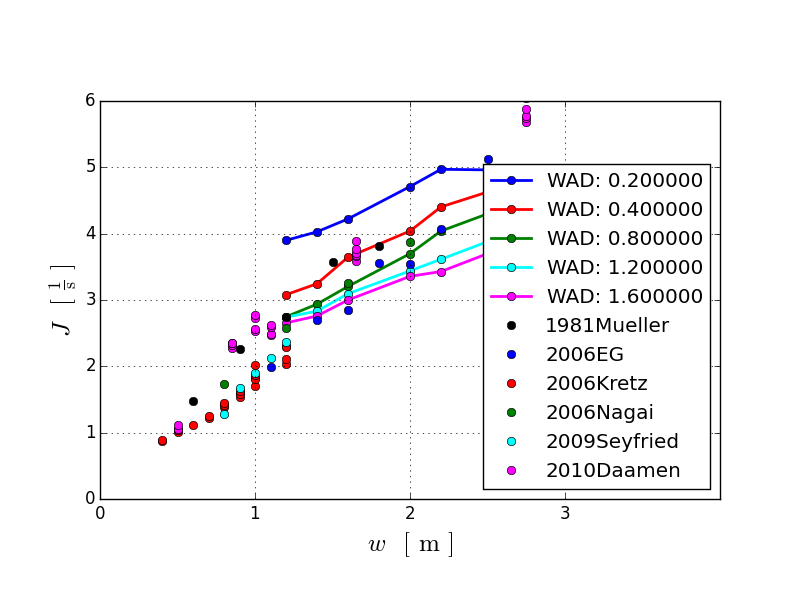
\includegraphics[width=1.\textwidth]{pics/sim_flow_vs_experimental_data}
\caption{Fundamental diagram with empiric data and simulation results}
\label{funddiag}
\end{figure}
\subsection{Laneformation}
\begin{figure}[h!]
\subfigure{\includegraphics[width=.49\textwidth]{pics/corner0}}
\subfigure{\includegraphics[width=.49\textwidth]{pics/corner1}}
\subfigure{\includegraphics[width=.49\textwidth]{pics/corner2}}
\subfigure{\includegraphics[width=.49\textwidth]{pics/corner3}}
\subfigure{\includegraphics[width=.49\textwidth]{pics/corner4}}
\subfigure{\includegraphics[width=.49\textwidth]{pics/corner5}}
\caption{Bottleneck-Corner Experiment: After the bottleneck, agents pass the corner.}
\label{funddiag}
\end{figure}
\newpage
\section{Conclusion and Outlook}

In this thesis, an altered usage of an enhanced floor-field was shown, integrated in a suitable new TEST-model. The \emph{wall-avoid-distance} parameter was analyzed and shown to be able to show good convergence to empirical data. During the course of the work process, it became clear how versatile and powerful floor-fields can be. Not only in the current state, they can provide valuable assistance to pedestrian models, but they can be further developed to fit into much more contexts.

\subsection{Floor-field}

\subsubsection{Multiple Goals }

The floor-field is a useful tool in routing of pedestrians through any geometry. To unfold its full power, one can imagine to calculate a floor-field for each of many atomic goals\footnote{An atomic goal would be a single exit door, whereas a destination could consists of a set of doors/exits.}. The combination of many floor-fields, each corresponding to an atomic goal, can easily be managed by selecting the direction vector of the one floor-field, that provides the minimal time-cost of an active set of floor-fields evaluated at the grid-point of the current agent's position. Dynamic in-world events in a simulation could alter the set of active floor-fields. This way, models can implement navigation in a dynamically changing world. It can be also used, to be a tool in a simulation suit, which has agents change their destination during runtime. This would be realized by simply changing the active set to the floor-fields corresponding to the new destination.

<< Verteilerebene(?) oder etwas kleinere Geometrie mit mehreren Ausgaengen: Nebeneinander 2-4 Vectorfelder nebeneinander >>

\subsubsection{Multiple Floors}

In the current state, the floor-field provides time-cost on a discrete grid, a rectangular grid with equidistant spacing in each dimension. The grid-points are stored in a one-dimensional array by the row-major order. In a arrangement like this, it is easy to formulate 4-neighboring\footnote{Grid-points north, south, east and west to the current are called 4-neighbors.} relations.  These values are easily accessed, if you are provided the stride value, namely how much grid-points make up the length of both dimensions in a 2-D world. The Fast-Marching algorithm needs the time-cost values of the 4-neighborhood.
This will change, if you need to simulate in a building with multiple floors, which are connected via stairs. We need to introduce a third dimension, which can be treated equally handy inside each floor. Any position, projected onto the x-y-plane, may not be unique anymore. On the other hand, it would be a waste of memory, if a third dimension would be introduced\footnote{As we are interested in points representing the floor of a room, all the volume (air) above would be not used.} introduced, to represent the hull-cube circumscribing a building.
One is to find a solution, which describes the geometry of the rooms in a memory-efficient way and yet be able to comfortably access the 4-neighbors' time-cost value.

%\subsection{Usage in JuPedSim}

%\subsection{Floor-fields in Triangulated Domains}

%\subsection{Parallelization}
\newpage
\section{Appendices}

\subsection{Fast-Marching Algorithm}


\begin{sequencediagram}
\newthread[white]{u}{User}
\newinst[2]{f}{FloorfieldViaFM}
\newinst[5]{t}{Trial}

  \begin{call}{u}{Create and Init(...)}{f}{}
	\begin{call}{f}{Create and Init(...)}{t}{}
	\end{call}
	\begin{call}{f}{All points are marked unknown}{t}{}
	\end{call}
	\begin{call}{f}{Add target points to narrowband}{t}{}
	\end{call}

    \begin{sdblock}{while narrowband not empty}{}

     \begin{call}{f}{remove minimum from narrowband}{t}{}
     \end{call}
     \begin{callself}{f}{add minimum to know-set}{}{}
     \end{callself}
     \begin{callself}{f}{calc cost of minimum's unknown neighs}{}{}
     \end{callself}
     \begin{call}{f}{add unknown neighbors to narrowband}{t}{}
     \end{call}
   \end{sdblock}
   \begin{callself}{f}{save floorfield}{}{}
   \end{callself}
  \end{call}
\end{sequencediagram}
\newpage
\subsection{Gradient Model using a Floorfield}
\begin{adjustbox}{width=\textwidth, height=\textheight, keepaspectratio}
\begin{sequencediagram}
\newthread[white]{u}{User}
\newinst[2]{g}{GradientModel}
\newinst[2]{d}{DirectionStrategy}
\newinst[2]{f}{FloorfieldViaFM}

\begin{call}{u}{Create and Init(...)}{g}{}


\begin{call}{u}{Create and Init(...)}{d}{}
   \begin{call}{d}{Create and Init(...)}{f}{}
   \begin{sdblock}{run simulation}{} 
     \begin{callself}{g}{for each agent}{}{}
       \begin{call}{g}{getTarget()}{d}{return movDir}
         \begin{call}{d}{getDirectionAt()}{f}{return movDir}
         \end{call}
       \end{call}
       
       \begin{call}{g}{getDir2Wall()}{d}{return dir2Wall}
         \begin{call}{d}{getDir2Wall()}{f}{return dir2Wall}
         \end{call}
       \end{call}
       
       \begin{call}{g}{getDistance2Wall()}{d}{return distance2Wall}
         \begin{call}{d}{getDistance2Wall()}{f}{return distance2Wall}
         \end{call}
       \end{call} 
       \begin{callself}{g}{calc moving vector}{}{}
       \end{callself}      
     \end{callself}
   \end{sdblock}
  \end{call}
  \end{call}
\end{call}
\end{sequencediagram}
\end{adjustbox}
\newpage
%\subsection{Code Snippets}
\setstretch{1}
%\lstinputlisting[label=FFviaFM_h,caption=FloorfieldViaFM Class Header]{../../routing/FloorfieldViaFM.h}
\newpage
%\lstinputlisting[label=RectGrid,caption=RectGrid Class Header]{../../routing/mesh/RectGrid.h}
\newpage
%\section{Bibliography}

\bibliographystyle{plain}

\addcontentsline{toc}{section}{Literatur}
\bibliography{masterthesisArGr}

%micro-/macroscopic arbeiten (desktop/READ)

%fast-marching arbeiten:
%madrid
%code

%outlook: triangulated version (master/pdfs/fmarcher)

%Helbing and Moln�r 1995, Hartmann 2010, Hartmann et al. 2012, ( + Felix 4.2)

%history: helbing, ... (einleitungen von mc, uk, fd)

\end{document}